\documentclass{article}

\usepackage{amssymb}
\usepackage{amsmath}
\usepackage[swedish]{babel}
\usepackage{tikz}
\usepackage{pgfplots}
\usepackage{xcolor}
\usepgfplotslibrary{fillbetween}
\pgfplotsset{compat=1.18}

\definecolor{myblue}{RGB}{40,100,200}
\definecolor{myred}{RGB}{200,60,60}
\definecolor{mygreen}{RGB}{33,151,0}

\title{Integralkriteriet}
\author{Marcus Persson}
\date{\today}

\begin{document}
\maketitle

\section*{\underbar{Cauchy's Integralkriterie, sats 7.1:}}

Antag att $f$ är en positiv, avtagande och kontinuerlig funktion på intervallet $I=[1,\infty)$, då följer:

\begin{flalign*}
    &\sum_{k=1}^{\infty} f(k) \text{ konvergerar om och endast om}\\
    &\int_{1}^{\infty} f(x)\,dx \text{ konvergerar} &&
\end{flalign*}

\section*{\underbar{Sats}}

Antag att vi har en serie:

\begin{equation*}
    \sum_{k=1}^{\infty}f(k)
\end{equation*}

\noindent Där $f$ är en avtagande och kontinuerlig funktion på intervallet, $I=[1,\infty)$

% Graph for visual understanding
\begin{figure}[ht]
    \centering
    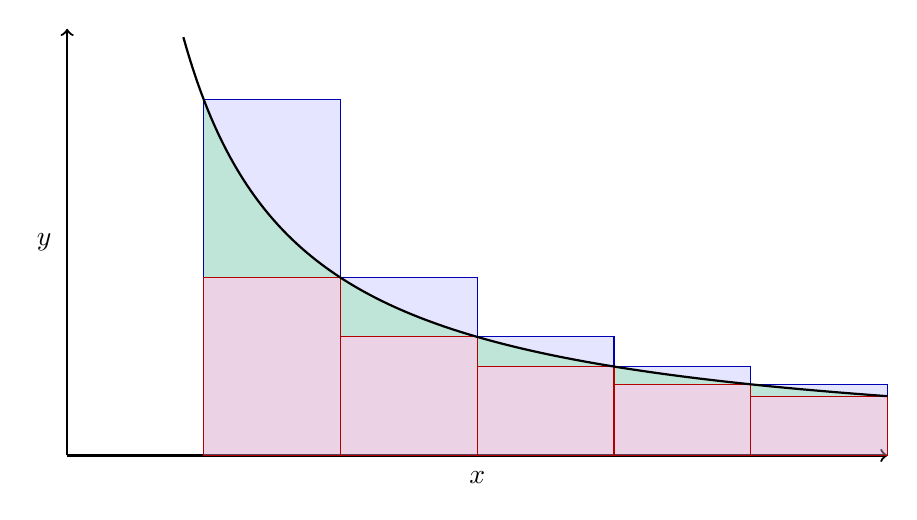
\begin{tikzpicture}
        \begin{axis}[
            xmin=0, xmax=6,
            ymin=0, ymax=1.2,
            axis lines=left,
            axis line style={->, thick},
            xtick=\empty,
            ytick=\empty,
            xlabel={$x$},
            ylabel={$y$},
            ylabel style={rotate=-90},
            width=12cm,
            height=7cm,
            clip=false
        ]

        % Left endpoint rectangles

        % Green areas between lower rectangles and function
        \foreach \a/\b/\h in {
            1/2/0.5,
            2/3/0.333333,
            3/4/0.25,
            4/5/0.2,
            5/6/0.166667
        } {
            \addplot[
                draw=none,
                domain=\a:\b,
                name path=curve,
                forget plot
            ] {1/x};

            \addplot[
                draw=none,
                domain=\a:\b,
                name path=lower,
                forget plot
            ] {\h};

            \addplot[
                green!50,
                fill opacity=0.4,
                draw=none
            ] fill between[
                of=curve and lower
            ];
        }

        % Upper estimate (left endpoints)
        \path[draw=blue!70!black, fill=blue!40, fill opacity=0.25]
            (axis cs:1,0) rectangle (axis cs:2,1);
        \path[draw=blue!70!black, fill=blue!40, fill opacity=0.25]
            (axis cs:2,0) rectangle (axis cs:3,0.5);
        \path[draw=blue!70!black, fill=blue!40, fill opacity=0.25]
            (axis cs:3,0) rectangle (axis cs:4,0.3333);
        \path[draw=blue!70!black, fill=blue!40, fill opacity=0.25]
            (axis cs:4,0) rectangle (axis cs:5,0.25);
        \path[draw=blue!70!black, fill=blue!40, fill opacity=0.25]
            (axis cs:5,0) rectangle (axis cs:6,0.2);

        % Lower estimate (right endpoints)
        \path[draw=red!70!black, fill=red!40, fill opacity=0.25]
            (axis cs:1,0) rectangle (axis cs:2,0.5);
        \path[draw=red!70!black, fill=red!40, fill opacity=0.25]
            (axis cs:2,0) rectangle (axis cs:3,0.3333);
        \path[draw=red!70!black, fill=red!40, fill opacity=0.25]
            (axis cs:3,0) rectangle (axis cs:4,0.25);
        \path[draw=red!70!black, fill=red!40, fill opacity=0.25]
            (axis cs:4,0) rectangle (axis cs:5,0.2);
        \path[draw=red!70!black, fill=red!40, fill opacity=0.25]
            (axis cs:5,0) rectangle (axis cs:6,0.1667);

        % Function
        \addplot[
            domain=0.85:6,
            samples=200,
            thick,
            black
        ] {1/x};

        \end{axis}
    \end{tikzpicture}
    \caption{}
    \label{fig:integral-criterion}
\end{figure}

\noindent Enligt figur (\ref{fig:integral-criterion}) får vi då:

\begin{equation*}
    \textcolor{myred}{\sum_{k=2}^{n}f(k)} \leq
    \textcolor{mygreen}{\int_{1}^{n}f(x)} \leq
    \textcolor{myblue}{\sum_{k=1}^{n-1}f(k)}
\end{equation*}

\noindent Detta medför att:

\begin{equation}
\label{EQ}
\tag{EQ}
    \int_{1}^{n}f(x)dx + f(n) \leq
    \sum_{k=1}^{n}f(k) \leq
    \int_{1}^{n}f(x)dx + f(1)
\end{equation}

\noindent Vi vill bevisa Cauchy's Integralkriterie med hjälp av (\ref{EQ})

\section*{\underbar{Bevis:}}

Låt $f \geq 0 \Rightarrow$ serien är positiv och den konvergerar om och endast om delsummorna är uppåtbegränsade. Eftersom $f\geq 0$ följer:

\begin{flalign*}
    &\int_{1}^{n}f(x)\,dx \text{ är en funktion beroende på }n\\
    &\text{Speciellt är } \int_{1}^{n}f(x)\,dx \text{ uppåtbegränsade om och endast om:}\\
    &\int_{1}^{\infty}f(x)\,dx \text{ är konvergent.}&&
\end{flalign*}

\noindent Då följer att delsummorna till $\sum_{k=1}^{n}f(k)$ är uppåtbegränsade av $\int_{1}^{n}f(x)\,dx + f(1)$ tack vare den högra olikheten i (\ref{EQ}).

\noindent Om serien är divergent blir delsummorna obegränsade enligt den vänstra olikheten i (\ref{EQ}) och serien blir då divergent.

\begin{flushright}
    $\blacksquare$
\end{flushright}

\end{document}